\documentclass[a4paper]{article}
\usepackage{fontspec}
\usepackage{amsmath}
\usepackage{amsfonts}
\usepackage{amssymb}
\usepackage{bm}
\usepackage{graphicx}
\usepackage{subcaption}
\usepackage[colorlinks=true,
linkcolor=blue,
citecolor=blue,
urlcolor=blue]
{hyperref}
\usepackage{cleveref}
\usepackage[left=1.00in, right=1.00in, top=1.00in, bottom=1.00in]{geometry}
\usepackage{booktabs}
\usepackage{lmodern}
\title{Introduction to Materials}
\author{Daniel Celis Garza}
\date{\today}
\begin{document}
\maketitle
	\section{Question 1}
	\subsection{a)}
	\subsubsection{i)}
		How many atoms in a BCC unit cell?
		
		\begin{figure}
			\centering
			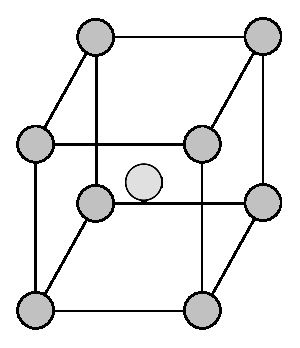
\includegraphics[width=0.33\linewidth]{bcc.eps}
			\caption{BCC unit cell.}
			\label{f:bcc}
		\end{figure}
		2 atoms per unit cell. $1/8$ atom per vertex, $1$ atom in the middle.
		
	\subsubsection{ii)}
		Estimate the density of Chromium (BCC) if the atomic radius, $R = 0.125$ nm, molar mass, $M = 52.0$ g/mol.
		
		\begin{figure}
			\centering
			\begin{subfigure}[b]{0.3\linewidth}
				\centering
				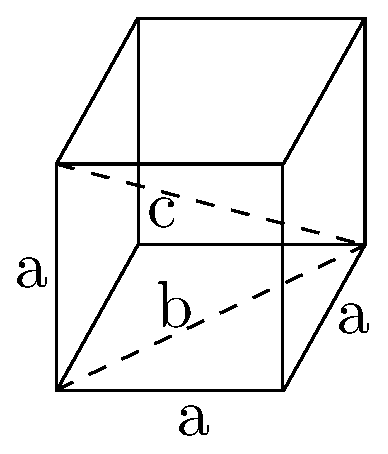
\includegraphics[width=\linewidth]{diag.eps}
				\caption{Cube diagonals.}
				\label{sf:diag}
			\end{subfigure}
			~
			\begin{subfigure}[b]{0.3\linewidth}
				\centering
				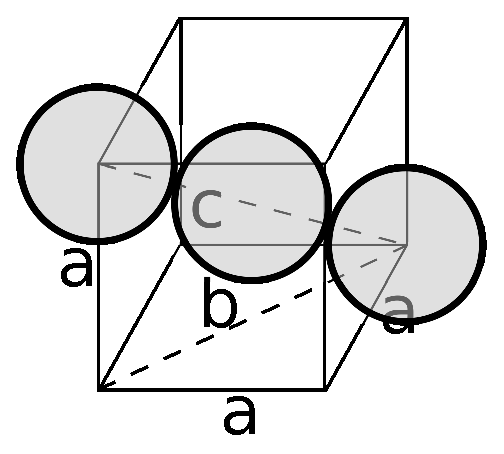
\includegraphics[width=\linewidth]{diag2.eps}
				\caption{Main diagonal (space filling).}
				\label{sf:diag2}
			\end{subfigure}
			~
			\begin{subfigure}[b]{0.3\linewidth}
				\centering
				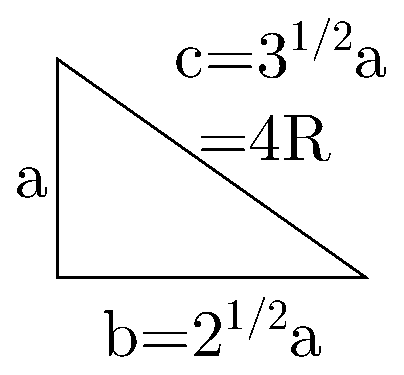
\includegraphics[width=\linewidth]{triag.eps}
				\caption{Diagonal values.}
				\label{sf:diag3}
			\end{subfigure}
			\label{f:diag}
		\end{figure}
		Density,
		\begin{align}
			\rho = m/v~, \label{e:dens}
		\end{align}
		where $m \equiv $ mass and $v \equiv $ volume. From \cref{f:diag} we find,
		\begin{align}
			a &= \dfrac{4}{\sqrt{3}} R \\
			v_{\textrm{unit cell}} &= a^{3} = \left(\dfrac{4}{\sqrt{3}}\right)^{3} R^{3}~, \label{e:volume}
		\end{align}
		The mass of a BCC metal in a unit cell, 
		\begin{align}
			m_{\textrm{unit cell}} = M \times \dfrac{2}{A_{N}}, \label{e:mass}
		\end{align} 
		where $2 \equiv $ number of atoms in a unit cell and $A_{N} \equiv $ avogadro's constant. Substituting \cref{e:volume, e:mass} into \cref{e:dens} we obtain an expression for the density of any BCC metal using values for its unit cell,
		\begin{align}
			\rho = \dfrac{2 \sqrt{3^{3}} M }{4^{3} R^{3} A_{N}}~.
		\end{align}
		Substituting the relevant values we find \cref{se:rho},
		\begin{subequations}
		\begin{align}
			\rho &= \dfrac{2 \sqrt{27} \times 52.0}{4^{3} \left(0.125 \times 10^{-7} \right)^{3} 6.022 \times 10^{23} \textrm{atom/mol}} \dfrac{[\textrm{atom g mol$^{-1}$}]}{[\textrm{atom cm$^{3}$ mol$^{-1}$}]}\\
			     &= 7.18 \textrm{ g/cm$^{3}$} \label{se:rho}\\
			\rho_{\textrm{real}} &= 7.15 \textrm{ g/cm$^{3}$}~.
		\end{align}
		\end{subequations}
		
		\subsection{b)}
		\subsubsection{i)}
		Given, 
		\begin{align}
			v_{1} &= \begin{bmatrix}
					1 & 2 & 3
					\end{bmatrix}\\
			v_{2} &= \begin{bmatrix}
					1 & 1 & -1
					\end{bmatrix}\\
			v_{3} &= \begin{bmatrix}
					1 & 1 & 1
					\end{bmatrix}~.
		\end{align}
		Show $v_{1} \parallel v_{2}$ and $v_{1} \not\parallel v_{3}$.
		
		By the dot product,
		\begin{subequations}		
		\begin{align}
			v_{1} \cdot v_{2} &= \begin{bmatrix}
								1 & 2 & 3
								\end{bmatrix} 
								\begin{bmatrix}
								1\\
								1\\
								-1
								\end{bmatrix}
							    = 1 + 2 - 3 = 0\\
			v_{1} \cdot v_{3} &= \begin{bmatrix}
								1 & 2 & 3
								\end{bmatrix} 
								\begin{bmatrix}
								1\\
								1\\
								1
								\end{bmatrix}
								= 1 + 2 + 3 = 6~.
		\end{align}
		\end{subequations}
	\subsubsection{ii)}
	The zone axis refers to translational invariance between planes. They're described as integer basis vectors such that translations by the basis vector can move any plane to another with the same zone axis. Essentially they are a linear map $f: R^{2} \to R^{2'}$, $f$ being the zone axis. Represented here as the trace of a $3\times3$ matrix.
	\begin{align}
		\begin{bmatrix}
		u & v & w
		\end{bmatrix} &\to 
		\begin{bmatrix}
		u' & v' & w'
		\end{bmatrix}\\
		\begin{bmatrix}
		u & v & w
		\end{bmatrix}
		\begin{bmatrix}
		a & 0 & 0\\
		0 & b & 0 \\
		0 & 0 & c
		\end{bmatrix}
		&=
		\begin{bmatrix}
		u' & v' & w'
		\end{bmatrix}~.
	\end{align}
	\subsubsection{iii)}
	The indices of zone axis can be found by simple vector subtraction of the parallel plane, and multiplying by the smallest factor so all numbers are integer values.
	\begin{align}
		v_{1} - v_{2} = 
		\begin{bmatrix}
		0 & 1 & 4
		\end{bmatrix}~.
	\end{align}
	
	\subsection{c)}
	Cu$_{3}$Au has an FCC lattice. If the collection of atoms is translated to all vertices of the unit cell we obtain an FCC lattice (\cref{f:fcc}).
	\begin{figure}
		\centering
		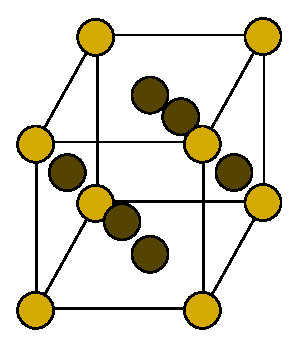
\includegraphics[width=0.33\linewidth]{cu3au.eps}
		\caption{FCC Cu$_{3}$Au unit cell.}
		\label{f:fcc}
	\end{figure}
	\subsection{d)}
	Ni has an FCC unit cell. From \cref{f:fcc} we see that the crystallographic direction for the nearest neighbours are,
	\begin{align}
		\begin{bmatrix}
		\dfrac{1}{2} & \dfrac{1}{2} & 0
		\end{bmatrix},~
		\begin{bmatrix}
		\dfrac{1}{2} & 0 & \dfrac{1}{2}
		\end{bmatrix},~
		\begin{bmatrix}
		0 & \dfrac{1}{2} & \dfrac{1}{2}
		\end{bmatrix},~
	\end{align}
	and the second nearest neighbours,
	\begin{align}
		\begin{bmatrix}
		1 & 0 & 0
		\end{bmatrix},~
		\begin{bmatrix}
		0 & 1 & 0
		\end{bmatrix},~
		\begin{bmatrix}
		0 & 0 & 1
		\end{bmatrix}.
	\end{align}
	\subsection{e)}
	Hexagonal close-packed structures can be represented by translating only two atoms throughout the primitive lattice. \Cref{f:hcp2d} shows the 2D projection of the HCP primitive lattice to illustrate the idea.
	\begin{figure}
		\centering
		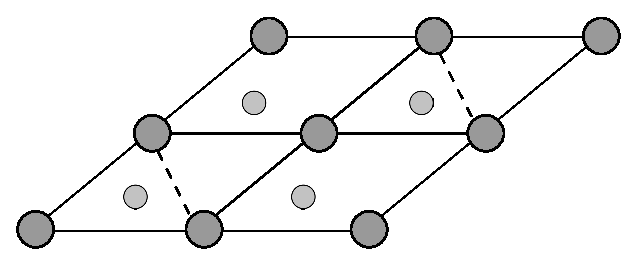
\includegraphics[width=0.33\linewidth]{hcp2d.eps}
		\caption{2D projection of HCP lattice showing how only two atoms need to be translated between lattice points to produce the structure. Smaller atoms lie on planes lower than the bigger ones. Dashed lines represent the non-primitive hexagonal unit cell.}
		\label{f:hcp2d}
	\end{figure}
	
	\section{Question 2}
	For diffraction to occur, the difference in distance travelled by both rays must be an integer multiple of the X-ray wavelength. Otherwise destructive interference will annihilate them both. From \cref{f:xraydiff} we know,
	\begin{subequations}
		\begin{align}
			n \lambda &= AB + BC - AD  \\
			AB &= BC = \dfrac{d}{\sin(\theta)} \\
			AC &= \dfrac{2 d}{\tan(\theta)} \\
			AD &= AC \cos(\theta) = \dfrac{2 d \cos^{2}(\theta)}{\sin(\theta)} \\
			n \lambda &= \dfrac{2 d}{\sin(\theta)} - \dfrac{2 d}{\sin(\theta)} \cos^{2}(\theta) \\
			n \lambda &= \dfrac{2 d}{\sin(\theta)} \left(1 - \cos^{2}(\theta)\right) \\
			n \lambda &= \dfrac{2 d}{\sin(\theta)} \sin^{2}(\theta) \\
			n \lambda &= 2 d \sin(\theta)~.
		\end{align}
	\end{subequations}
	Because we're in cubic symmetry we can use the Euler norm to find the inter planar distance,
	\begin{align}
		d = \dfrac{a}{\sqrt{h^{2} + k^{2} + l^{2}}}~.
	\end{align}
	Ignoring higher frequency harmonics and defining $N = h^{2} + k^{2} + l^{2}$ we arrive at,
	\begin{align}
		\lambda = \dfrac{2a}{\sqrt{N}} \sin(\theta)~.
	\end{align}
	\begin{figure}
		\centering
		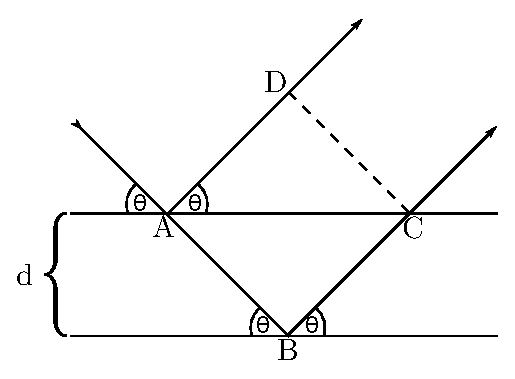
\includegraphics[width=0.33\linewidth]{bragg.eps}
		\caption{Schematic of X-ray diffraction.}
		\label{f:xraydiff}
	\end{figure}
	\subsection{b)}
	The structure factor gives information on the amplitudes and phase of the diffracted beams,
	\begin{align}
		F_{hkl} = \sum\limits_{i=1}^{N} f_{i} \exp\left[ -2 \pi i (h x_{i} + k y_{i} + l z_{i}) \right]~,
	\end{align}
	where $i$ represents an atom, $x_{i},~ y_{i},~ z_{i}$ are the coordinates of the basis atoms that comprise the primitive unit cell, and $h,~ k,~ l$ are a plane's miller indices, and $f_{i}$ is the scattering factor for the $i$'th atom. For certain planes, the structure factor vanishes completely and as a result, the intensity of the refracted beam is zero for such planes. This leads to a systematic absence of planes, and therefore the selection rules as seen in the lecture course.
	
	\subsection{c)}
	Using an X-ray $\lambda = 0.1524$ nm, on a cubic crystal powder.
	\subsubsection{i)}
	\Cref{t:diff} shows the refracting planes.
	\begin{table}
		\centering
		\caption{Diffraction table with crystal planes.}
		\label{t:diff}
		\begin{tabular}{cccccc}
			\toprule
			$2\theta$ & $\theta$ & $\sin^{2}\theta$ & $N = \sin^{2}\theta/R$ & $h,~ k,~ l$ & $ R = \sin^{2}\theta/N $\\
			\midrule
			$28.2$ & $14.1$  & $0.059$ & $3$  & $1,~1,~1$ & $ 0.0198 $ \\
			$32.7$ & $16.35$ & $0.079$ & $4$  & $0,~0,~2$ & $ 0.0198 $ \\
			$46.9$ & $23.45$ & $0.158$ & $8$  & $0,~2,~2$ & $ 0.0198 $ \\
			$55.6$ & $27.8$  & $0.218$ & $11$ & $1,~1,~3$ & $ 0.0198 $ \\
			$58.3$ & $29.15$ & $0.237$ & $12$ & $2,~2,~2$ & $ 0.0198 $ \\
			$68.4$ & $34.2$  & $0.316$ & $16$ & $0,~0,~4$ & $ 0.0198 $ \\
			$75.6$ & $37.8$  & $0.376$ & $19$ & $1,~3,~3$ & $ 0.0198 $ \\
			$77.9$ & $38.95$ & $0.395$ & $20$ & $0,~2,~4$ & $ 0.0198 $ \\
			$87.1$ & $43.55$ & $0.475$ & $24$ & $2,~2,~4$ & $ 0.0198 $ \\
			\bottomrule
		\end{tabular}
	\end{table}
	\subsubsection{ii)}
	The lattice parameter $a$, is given by,
	\begin{subequations}
		\begin{align}
			a &= \dfrac{\lambda}{2 \sqrt{R}}\\
			  &= \dfrac{0.1524}{2 \sqrt{0.0198}} = 0.5404 \textrm{ nm}~.
		\end{align}
	\end{subequations}
	
	\section{Question 3}
	\subsection{a)}
	The root mean squared free path is given by,
	\begin{align}
		x_{rms} = \sqrt{D t}~,\label{e:rms}
	\end{align}
	where $D \equiv $ diffusivity and $t \equiv$ time. Assuming the diffusivity to be an activated process we have,
	\begin{align}
		D = D_{0} \exp\left(-\dfrac{Ea}{RT}\right)~,\label{e:diff}
	\end{align}
	where $Ea \equiv$ activation energy, $R \equiv $ ideal gas constant and $T \equiv$ temperature. Plugging \cref{e:diff} into \cref{e:rms},
	\begin{align}
		x_{rms} = \sqrt{D_{0} \exp\left(-\dfrac{Ea}{RT}\right) t}~.\label{e:rmsdiff}
	\end{align}
	
	First we need to find $D_{0}$ for the known scenario $x_{rms} = 0.5 \textrm{ mm},~ T = 293.15 \textrm{ K},~ Ea = 30 \text{ kJ},~ R = 8.314 \text{ J mol$^{-1}$ K$^{-1}$ }$,
	\begin{subequations}
	\begin{align}
		D_{0} &= \dfrac{0.5^{2} \exp\left(\dfrac{30 \times 10^{3}}{8.314 \times 293.15}\right) }{30} \dfrac{\textrm{[mm$^2$]}}{\textrm{[min]}}\\
			  &= 1847.28 \textrm{ mm$^2$ min$^{-1}$}.~
	\end{align}
	\end{subequations}
	We then solve for $t$ at $T = 353.15 \textrm{ K}$,
	\begin{subequations}
	\begin{align}
		t &= \dfrac{0.5^{2} \exp\left(\dfrac{30 \times 10^{3}}{8.314 \times 353.15}\right) }{1847.28} \dfrac{\textrm{[mm$^2$]}}{\textrm{[mm$^2$ min$^{-1}$]}}\\
		  &= 3.706 \textrm{ min}
	\end{align}
	\end{subequations}
	\subsection{b)}
	Edge dislocations are concerted movements of lines of atoms perpendicular to the Burger's vector. As a result, the dislocation moves parallel to the vector because subsequent perpendicular lines of atoms become displaced. Screw dislocations are concerted movements of lines of atoms parallel to the Burgers vector. As more parallel lines of atoms become displaced, the dislocation moves perpendicular to the Burgers vector. \Cref{f:dis} shows both dislocation types and their movement.
	\begin{figure}
		\centering
		\begin{subfigure}[b]{0.45\linewidth}
			\centering
			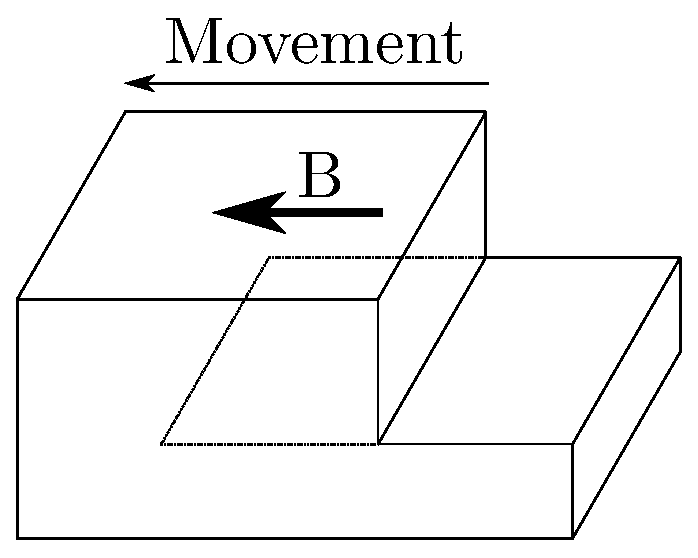
\includegraphics[scale=0.5]{edgedis.eps}
			\caption{Edge dislocation.}
		\end{subfigure}
		~
		\begin{subfigure}[b]{0.45\linewidth}
			\centering
			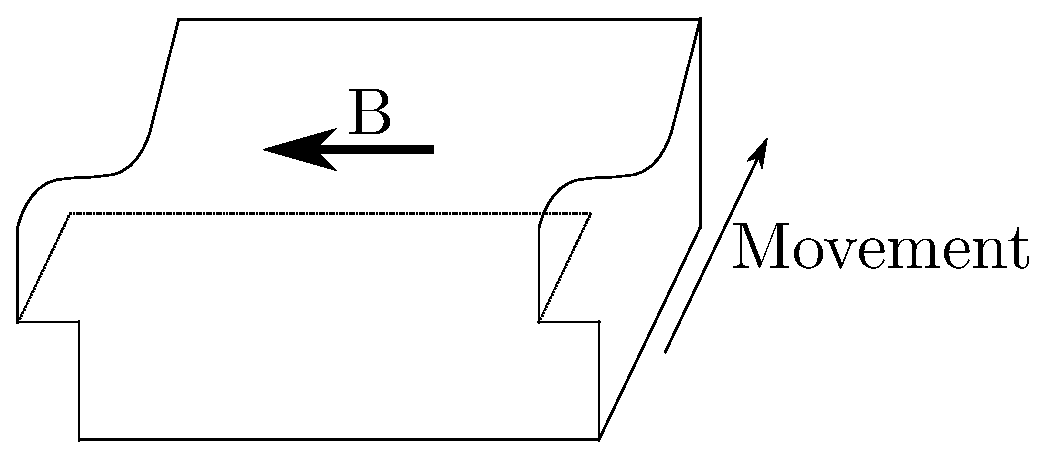
\includegraphics[scale=0.5]{screwdis.eps}
			\caption{Screw dislocation.}
		\end{subfigure}
		\caption{Dislocation types. Burger's vector is denoted by $B$.}
		\label{f:dis}
	\end{figure}
	\subsection{c)}
	The dislocation can be decomposed as follows,
	\begin{align}
		\dfrac{a}{2}
		\begin{bmatrix}
		1 & \overline{1} & 0 
		\end{bmatrix}
		\to
		\dfrac{a}{6}
		\begin{bmatrix}
		2 & \overline{1} & \overline{1} 
		\end{bmatrix}
		+
		\dfrac{a}{6}
		\begin{bmatrix}
		\overline{1} & 2 & \overline{1} 
		\end{bmatrix}~.
	\end{align}
	The dislocation energy is proportional to the modulus of each dislocation. A single dislocation will split into two partial dislocations if the energy of the two partials plus the stacking fault energy, $E_{s}$, is less than the energy of a full dislocation,
	\begin{subequations}
	\begin{align}
		\dfrac{a^{2}}{4} 
		\begin{bmatrix}
			1 & -1 & 0 
		\end{bmatrix}
		\begin{bmatrix}
		1\\ -1\\ 0 
		\end{bmatrix} 
		&\overset{?}{=}
		\dfrac{a^{2}}{36}
		\begin{bmatrix}
		2 & -1 & -1
		\end{bmatrix}
		\begin{bmatrix}
		2 \\ -1 \\ -1
		\end{bmatrix}
		+
		\dfrac{a^{2}}{36}
		\begin{bmatrix}
		-1 & 2 & -1
		\end{bmatrix}
		\begin{bmatrix}
		-1\\ 2 \\ -1
		\end{bmatrix}
		+ E_{s}\\
		\dfrac{a^{2}}{2} &\overset{?}{=} \dfrac{a^{2}}{3} + E_{s}~.
	\end{align}
	\end{subequations}
	The partial dislocations form an angle of $\frac{2}{3}\pi$ rad to each other.
	\subsection{d)}
	Radiation damage induces collision cascades that forcefully displace atoms creating so-called prismatic dislocation loops that---in contrast to edge and screw dislocations---move along cylindrical axes not on the plane of their Burgers vector. The damage also creates Fran-Read sources by creating stacking faults that are pinned in place by the prismatic loops or displaced atoms.
	
	\section{Question 4}
	\subsection{a)}
	It was found that the square root of a crack length, $a$, and the stress at the crack was nearly constant,
	\begin{align}
		\sigma \sqrt{a} \approx C~. \label{f:griffith1}
	\end{align}
	To find $C$ we need to recognise that two surfaces are created when a crack propagates. As a consequence, when a crack propagates, the elastic energy is reduced while surface energy is increased. By computing the energy difference, the following expression for $c$ can be found,
	\begin{align}
		c = \sqrt{\dfrac{2 E \gamma}{\pi}}~.
	\end{align}
	Failure occurs when the energy difference reaches a peak, beyond which it is lowered by increasing the crack length.
	\subsection{b)}
	\begin{figure}
		\centering
		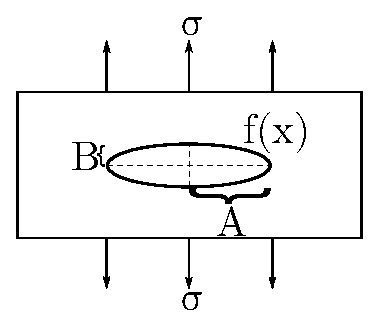
\includegraphics[width=0.33\linewidth]{griffderv.eps}
		\caption{Schematic of a crack.}
		\label{f:griffderv}
	\end{figure}
	We need to find an equation for a crack which is assumed to be a perfect ellipse as illustrated in \cref{f:griffderv}. We know the equation for an ellipse to be
	\begin{align}
		y = \dfrac{b}{a} \sqrt{a^{2} - x^{2}}~.
	\end{align}
	We also know the crack opening is proportional to the plane strain Young's modulus $E'$,
	\begin{align}
		E' = \dfrac{E}{1-\nu^{2}}~.
	\end{align}
	So we can assume our function from \cref{f:griffderv} to be
	\begin{align}
		f(x) = \dfrac{4 \sigma}{E'} \sqrt{a^{2} - x^{2}}~,
	\end{align}
	where the factor of $4$ comes from having each side of the crack (top and bottom) experiencing a total strain of $2 \sigma$.
	
	Assuming the stress energy released is equal to the surface energy of two crack surfaces forming, if we were to apply a stress $\sigma$ to close the crack, the energy needed would be
	\begin{subequations}
	\begin{align}
		E(a) &= \dfrac{\sigma}{2} \int\limits_{-a}^{a} f(x) \mathrm{d}x \\
			 &= \dfrac{2 \sigma^{2}}{E'} \int\limits_{-a}^{a} \sqrt{a^{2} - x^{2}} \mathrm{d}x \\
			 &= \dfrac{2 \sigma^{2}}{E'} \left[ \dfrac{1}{2} x \sqrt{a^{2} - x^{2}} + \dfrac{1}{2} a^{2} \arctan\left(\dfrac{x}{\sqrt{a^{2} - x^{2}}}\right) \right]_{-a}^{a}\\
			 &= \dfrac{\pi \sigma^{2} a^{2}}{E'}~.
	\end{align}
	\end{subequations}
	The energy released going from a crack of size $a \to a + \mathrm{d}x$ is
	\begin{align}
		\dfrac{\mathrm{d}E(a)}{\mathrm{d}a} &= \dfrac{2 \pi \sigma^{2} a}{E'}~.
	\end{align}
	According to our assumptions this is equal to the formation energy of two crack surfaces, $2G_{c}$, which after rearrangement gives the Griffith equation for a purely brittle fracture,
	\begin{align}
		\sigma &= \sqrt{\dfrac{G_{c} E'}{\pi a}}
	\end{align}
	\subsection{c)}
	\begin{enumerate}
		\item Stress concentration at the crack tip usually leads to localised plastic deformation. The plastic deformation leads to energy dissipation via heat thereby increasing the required energy for crack growth.
		\item Assuming sharp cracks means stress leads to infinity as crack radius tends to zero. In reality, this stress has a finite value because it is distributed all throughout the crack and into the surrounding plastic deformation zone.
		\item The model assumes linearity in resistance to crack growth. This assumption does not hold and the non-linearity depends on the plastic-elastic properties of the material as well as its geometry. Dislocation generation and motion plays a large role in this non-linear response.
	\end{enumerate}
	
	\section{Question 5}
	\subsection{a)}
	\begin{itemize}
		\item Slip plane: a plane that can move with relative ease compared to other planes in the material. Normally has the highest atom density.
		\item Slip direction: the direction that corresponds to the shortest lattice transition vectors. It is the preferred direction of movement of a slip plane.
		\item Slip system: the symmetrically identical set of slip planes and their associated slip directions.
	\end{itemize}
	\subsection{b)}
	\subsubsection{i)}\label{sss:csl}
	Because the energy associated with $ \{111\} \langle 1\overline{1}0 \rangle $ is lower than that for $ \{111\} \langle 001 \rangle $,
	\begin{subequations}
		\begin{align}
			\dfrac{a}{2}
			\begin{bmatrix}
			1 & -1 & 0
			\end{bmatrix}
			\dfrac{a}{2}
			\begin{bmatrix}
			1 \\ -1 \\ 0
			\end{bmatrix}
			&<
			a
			\begin{bmatrix}
			0 & 0 & 1
			\end{bmatrix}
			a
			\begin{bmatrix}
			0 \\ 0 \\ 1
			\end{bmatrix} \\
			\dfrac{a^{2}}{2} < a^{2}~.
		\end{align}
	\end{subequations}
	\subsubsection{ii)}
	In BCC iron the slip system is $ \{110\} \langle \overline{1}11 \rangle $.
	\subsection{c)}
	\begin{figure}
		\centering
		\begin{subfigure}[b]{0.35\linewidth}
			\centering
			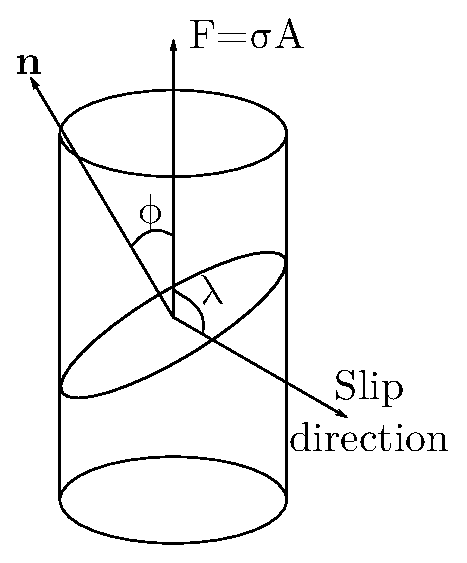
\includegraphics[width=\linewidth]{rstress.eps}
			\caption{Resolved shear stress diagram.}
		\end{subfigure}
		~
		\begin{subfigure}[b]{0.2\linewidth}
			\centering
			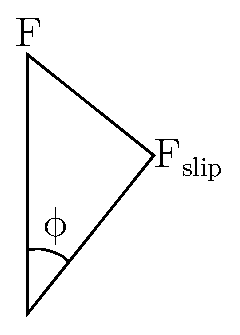
\includegraphics[width=\linewidth]{fslip.eps}
			\caption{$F_{\textrm{slip}}$ diagram.}
		\end{subfigure}
		~
		\begin{subfigure}[b]{0.35\linewidth}
			\centering
			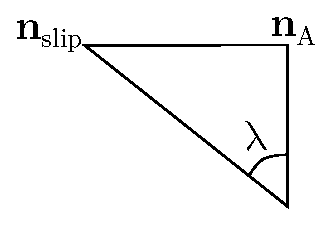
\includegraphics[width=\linewidth]{aslip.eps}
			\caption{$A_{\textrm{slip}}$ diagram.}
		\end{subfigure}
		\caption{Resolved shear stress.}
		\label{f:rstress}
	\end{figure}
	From \cref{f:rstress} we can obtain the following equations,
	\begin{subequations}
		\begin{align}
			\sigma &= \dfrac{F}{A} \\
			F_{\textrm{slip}} &= F \cos(\lambda) \\
			A_{\textrm{slip}} &= \dfrac{A}{\cos(\phi)} \\
			\sigma_{\textrm{slip}} &= \dfrac{F_{\textrm{slip}}}{A_{\textrm{slip}}} \\
			&= \sigma \cos(\lambda) \cos(\phi)~,
		\end{align}
	\end{subequations}
	where $\cos(\lambda) \cos(\phi)$ is the Schmidt factor.
	\subsection{d)}
	\subsubsection{i)}
	Schmidt's law states that the system on which slip occurs is that with the largest Schmidt factor, which is where $\phi = \lambda = \dfrac{\pi}{4} \therefore \cos^{2}\left(\dfrac{\pi}{4}\right) = \dfrac{1}{2}$.
	\subsubsection{ii)}
	Let $\bm{d}$ denote the direction of the applied stress $\sigma$. We know,
	\begin{align}
		\cos(\theta) &= \dfrac{\bm{a} \cdot \bm{b}}{\|a\| \|b\|}~.
	\end{align}
	Using the slip system for copper stated in \cref{sss:csl} we have,
	\begin{subequations}
		\begin{align}
			\cos(\phi) &= \dfrac{\bm{d}}{\|\bm{d}\|} \cdot \dfrac{\begin{Bmatrix} 1 & 1 & 1\end{Bmatrix}}{ \sqrt{3}}\\
			\cos(\lambda) &= \dfrac{\bm{d}}{\|\bm{d}\|} \cdot \dfrac{\langle\begin{matrix} 1 & \overline{1} & 0\end{matrix}\rangle}{\sqrt{2}}\\
			\sigma_{\textrm{slip}} &= \sigma \left(\bm{\hat{d}} \cdot \dfrac{\begin{Bmatrix} 1 & 1 & 1\end{Bmatrix}}{ \sqrt{3}}\right) \left(\bm{\hat{d}} \cdot \dfrac{\langle\begin{matrix} 1 & \overline{1} & 0\end{matrix}\rangle}{\sqrt{2}}\right)\\
			\sigma_{\textrm{slip}} &= \dfrac{\sigma}{\sqrt{6}} \left\|\bm{\hat{d}}\right\|^{2} \begin{Bmatrix} 1 & 1 & 1\end{Bmatrix} \cdot \langle\begin{matrix} 1 & \overline{1} & 0\end{matrix}\rangle~,
		\end{align}
	\end{subequations}
	where $\bm{\hat{d}}$ is the normalised direction of the stress.
	\subsection{d)}
	A tensile stress $\sigma$ is applied in the direction $\begin{bmatrix} 1 & -2 & 5\end{bmatrix}$.
	\subsubsection{i)}
	The slip factor for the slip system $(1 1 \overline{1})[1 0 1]$ is,
	\begin{subequations}
		\begin{align}
			\cos(\phi) &= \dfrac{\begin{bmatrix} 1 & -2 & 5 \end{bmatrix} \begin{bmatrix} 1 \\ 1 \\ -1 \end{bmatrix}}{
				\left(\begin{bmatrix}	1 & -2 & 5 \end{bmatrix} \begin{bmatrix} 1 \\ -2 \\ 5 \end{bmatrix}\right)
				\left(\begin{bmatrix}	1 & 1 & -1 \end{bmatrix} \begin{bmatrix} 1 \\ 1 \\ -1 \end{bmatrix}\right)
				} = \dfrac{-6}{30 \times 3} = -\dfrac{1}{15}\\
				\cos(\lambda) &= \dfrac{\begin{bmatrix} 1 & -2 & 5 \end{bmatrix} \begin{bmatrix} 1 \\ 0 \\ 1 \end{bmatrix}}{
					\left(\begin{bmatrix}	1 & -2 & 5 \end{bmatrix} \begin{bmatrix} 1 \\ -2 \\ 5 \end{bmatrix}\right)
					\left(\begin{bmatrix}	1 & 0 & 1 \end{bmatrix} \begin{bmatrix} 1 \\ 0 \\ 1 \end{bmatrix}\right)
				} = \dfrac{6}{30 \times 2} = \dfrac{1}{10}\\
			\cos(\phi) \cos(\lambda) &= -\dfrac{1}{150}
		\end{align}
	\end{subequations}
	\subsubsection{iii)}
	This is unlikely to be the most favoured slip system because the magnitude of this Schmidt factor is very small $<10^{-2}$, in fact the maximum magnitude for the Schmidt factor is 75 times greater than this. 
	
	\section{Question 6}
	\subsection{a)}
	Change in enthalpy of 1 mole of Ni heated from $25 ^{\circ}$ C to $225^{\circ}$ C. $C_{p} = 32.6 - 1.97 \times 10^{-3} T - 5.59 \times 10^{5} T^{-2} $ (J K$^{-1}$ mol$^{-1}$) is,
	\begin{subequations}
		\begin{align}
			\int\limits_{H_{0}}^{H} \textrm{d}H &= \int\limits_{T_{i}}^{T_{f}} C_{p} \mathrm{d}T\\
			\Delta H &= \int\limits_{298.15}^{428.15} \left(
			32.6 - 1.97 \times 10^{-3} T - 5.59 \times 10^{5} T^{-2}
			\right) \textrm{d}T \\
			\Delta H &= \left[32.6 T - \dfrac{1.97}{2} \times 10^{-3} T^{2} + 5.59 \times 10^{5} T^{-1}\right]_{298.15}^{498.15}\\
					 &= 3575.72~ \textrm{J mol$^{-1}$}~.
		\end{align}
	\end{subequations}
	\subsection{b)}
	\subsubsection{i)}
	\begin{itemize}
		\item Homogeneous nucleation: occurs within the liquid bulk in a random way, no catalyst is needed.
		\item Heterogeneous nucleation: occurs with the assistance of a catalyst, not fully random as it occurs on the catalyst surface. The catalyst can be an impurity precipitate, container wall, temperature fluctuation, etc. 
	\end{itemize}
	\subsubsection{ii)}
	Heterogeneous nucleation is most likely to occur in practice because perfect conditions are highly impractical and extremely unlikely to happen. It is much more likely that there are impurities, thermal variations and other factors which can act as nucleation seeds and catalysts.
	\subsection{c)}
	\Cref{f:nuc} is a sketch of a nucleation reaction over time. At stage I nucleation starts happening, slowly picking up speed as more and more nuclei start forming. At stage II the nucleation rate reaches an almost constant value as the thermodynamics dominate the reaction. At stage III the kinetics start becoming more important as there is progressively less material to nucleate, so the rate of nucleation decreases. At stage IV there is comparatively very little material left for nucleation and so many nuclei that they start aggregating into clumps, forming multicrystalline aggregates.
	\begin{figure}
		\centering
		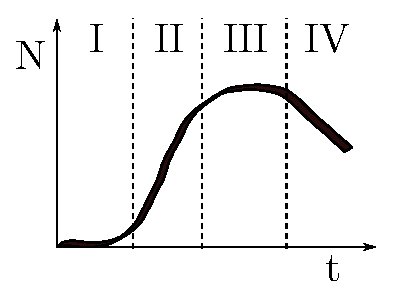
\includegraphics[width=0.33\textwidth]{nuc.eps}
		\caption{Stages of a nucleation reaction. I: Transient nucleation time. II: Steady-state nucleation regime. III: Decreased nucleation regime. IV: Coarsening regime.}
		\label{f:nuc}
	\end{figure}
	\subsection{d)}
	\Cref{f:ssol} shows the two types of solid solutions and provides an example of each one.
	\begin{figure}
		\centering
		\begin{subfigure}[b]{0.45\linewidth}
			\centering
			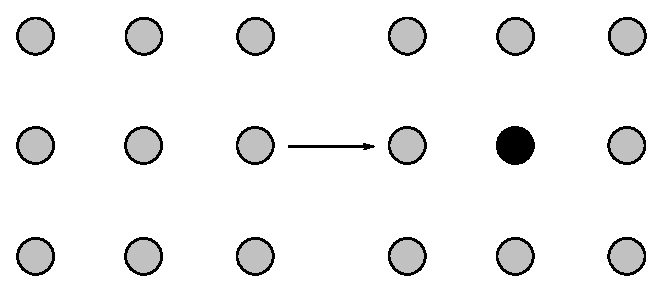
\includegraphics[width=\linewidth]{subs.eps}
			\caption{Substitutional: a solute atom substitutes a solvent atom in a lattice point. FCC Cu(Ni) is an example of a substitutional solid solution.}
			\label{sf:subs}
		\end{subfigure}
		\qquad\qquad
		\begin{subfigure}[b]{0.45\linewidth}
			\centering
			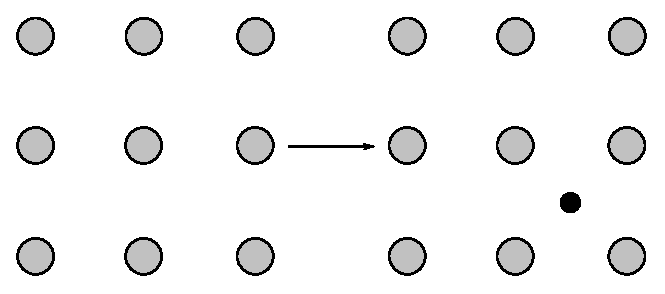
\includegraphics[width=\linewidth]{inters.eps}
			\caption{Interstitial: solute atoms lie in the interstices between solvent atoms. BCC Fe(C) is an example of an interstitial solid solution.}
			\label{sf:inters}
		\end{subfigure}
		\caption{Types and examples of solid solutions.}
		\label{f:ssol}
	\end{figure}
	\subsection{e)}
	\Cref{f:int} shows the types of interfaces and gives examples of each one.
	\begin{figure}
		\centering
		\begin{subfigure}[t]{0.3\linewidth}
			\centering
			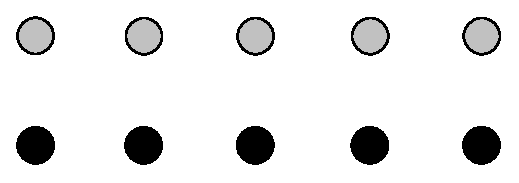
\includegraphics[width=\linewidth]{cohint.eps}
			\caption{Coherent interface: lattice sites remain undisturbed at the interface. Al/Al$_{2}$O$_{3}$ presents coherent and semicoherent interfaces.}
			\label{sf:cohint}
		\end{subfigure}
		~
		\begin{subfigure}[t]{0.3\linewidth}
			\centering
			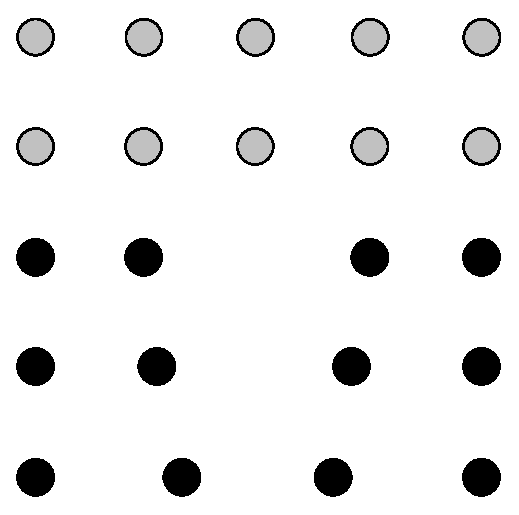
\includegraphics[width=\linewidth]{scohint.eps}
			\caption{Semicoherent interface: lattice sites are minimally disturbed at the interface, but return to normal a short distance away. Al/Al$_{2}$O$_{3}$ presents coherent and semicoherent interfaces.}
			\label{sf:scohint}
		\end{subfigure}
		~
		\begin{subfigure}[t]{0.3\linewidth}
			\centering
			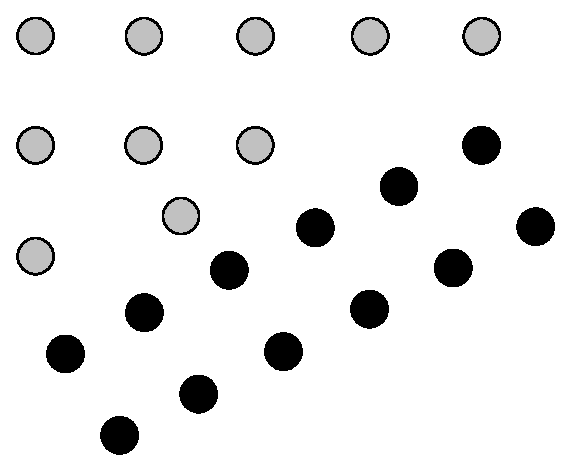
\includegraphics[width=\linewidth]{icohint.eps}
			\caption{Incoherent interface: lattice sites are completely disturbed, atoms may be missing from their site or displaced from it. ODS steels present incoherent interfaces.}
			\label{sf:icohint}
		\end{subfigure}
		\caption{Interface types and examples.}
		\label{f:int}
	\end{figure}
	
	\section{Question 7}
	\subsection{a)}
	The Hume-Rothery rules governing the formation of solid solutions by metal alloys are:
	\begin{itemize}
		\item atomic size factor---solubility is greater when atoms are of similar sizes since point substitutions are easier to achieve with similarly size atoms;
		\item electrochemical factor---solubility is greater when atoms have similar electronegativities because large differences favour the formation of intermetallic compounds;
		\item relative valence factor---low valency metals dissolve high valency metals better than vice-versa because lower valency metals have less localised electron clouds allowing for weaker and less directional bonds.
	\end{itemize}
	\subsection{b)}
	\Cref{f:steelpd} shows a sketch of the Fe-C phase diagram. In binary phase diagrams, invariant reactions happen vertically across a horizontal line where two other lines meet. In steel this only happens in three places. \Cref{e:fecr} shows the invariant reaction shown in the diagram.
	\begin{subequations}
		\begin{align}
			\textrm{Eutectic: } L &\leftrightarrow S_{1} + S_{2}, \quad &\textrm{L} &\leftrightarrow \gamma + \textrm{ledeburite}\\
			\textrm{Peritectic: } L + S_{1} &\leftrightarrow S_{2}, \quad &\textrm{L} + \delta &\leftrightarrow \gamma\\
			\textrm{Eutectoid: } S_{1} &\leftrightarrow S_{2} + S_{3}, \quad &\gamma &\leftrightarrow \alpha + \textrm{pearlite} \\
		\end{align}\label{e:fecr}
	\end{subequations}
	\begin{figure}
		\centering
		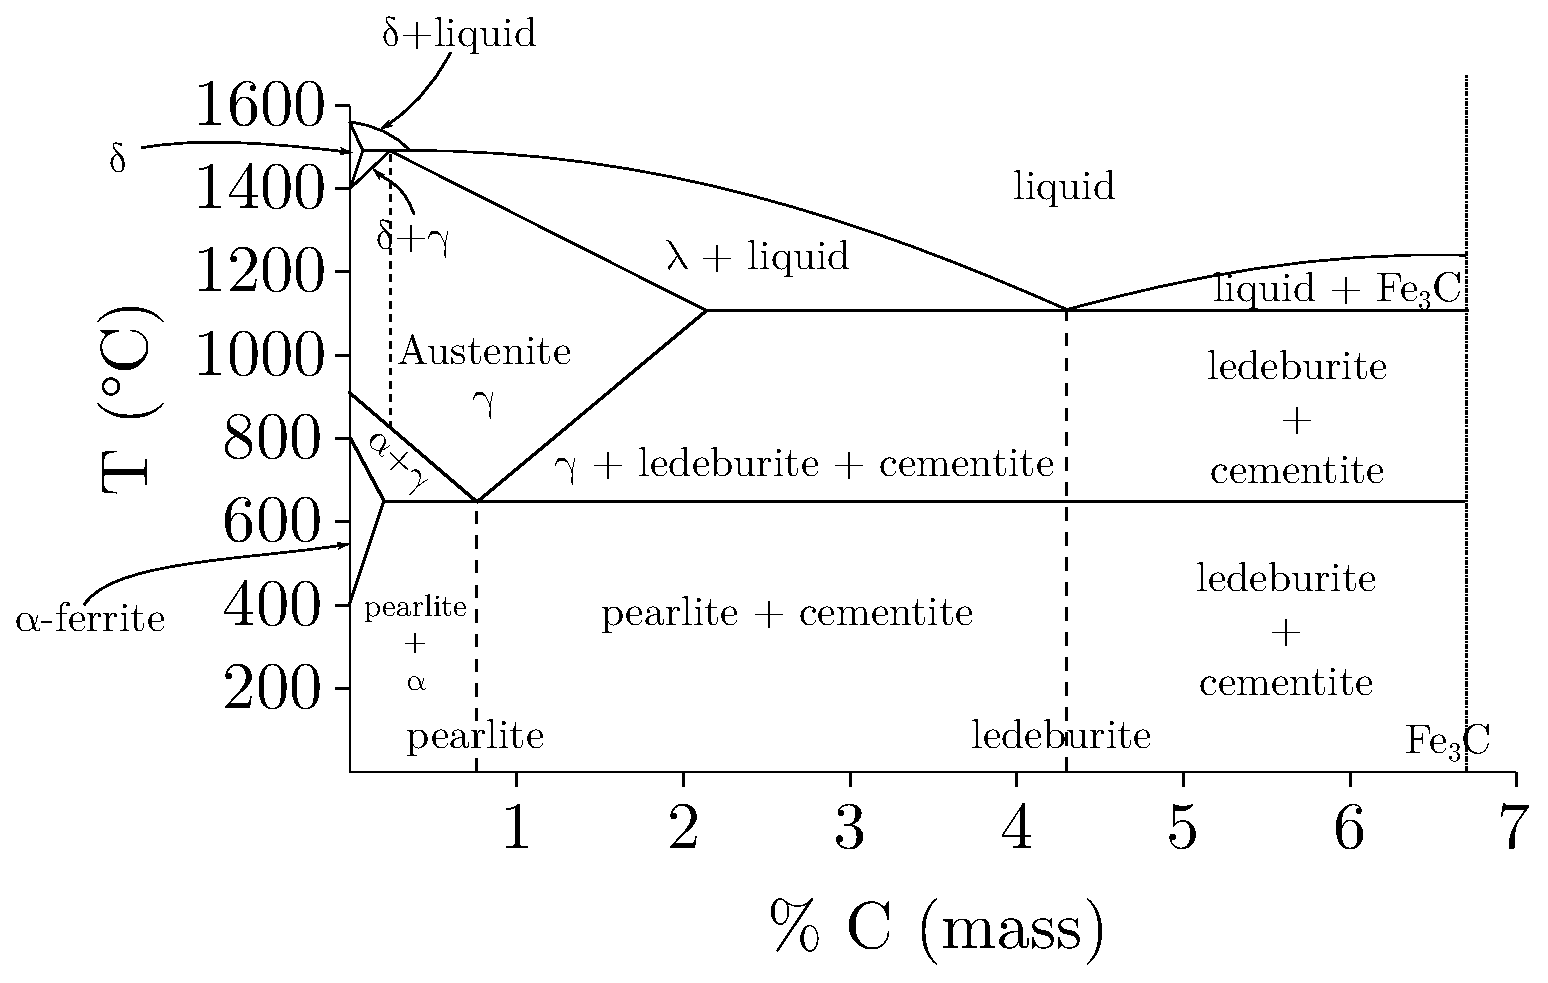
\includegraphics[width=\textwidth]{fecpd.eps}
		\caption{Fe-C phase diagram. Dashed lines show invariant reactions.}
		\label{f:steelpd}
	\end{figure}
	\subsection{c)}
	Martensite is a non-equilibrium phase of the Fe-C system created by rapid quenching. Since phase diagrams deal only with equilibrium species, martensite does not show up.
	\subsection{d)}\label{ss:pdab}
	\Cref{f:pdab} shows a sketch of a labelled binary phase diagram.
	\begin{figure}
		\centering
		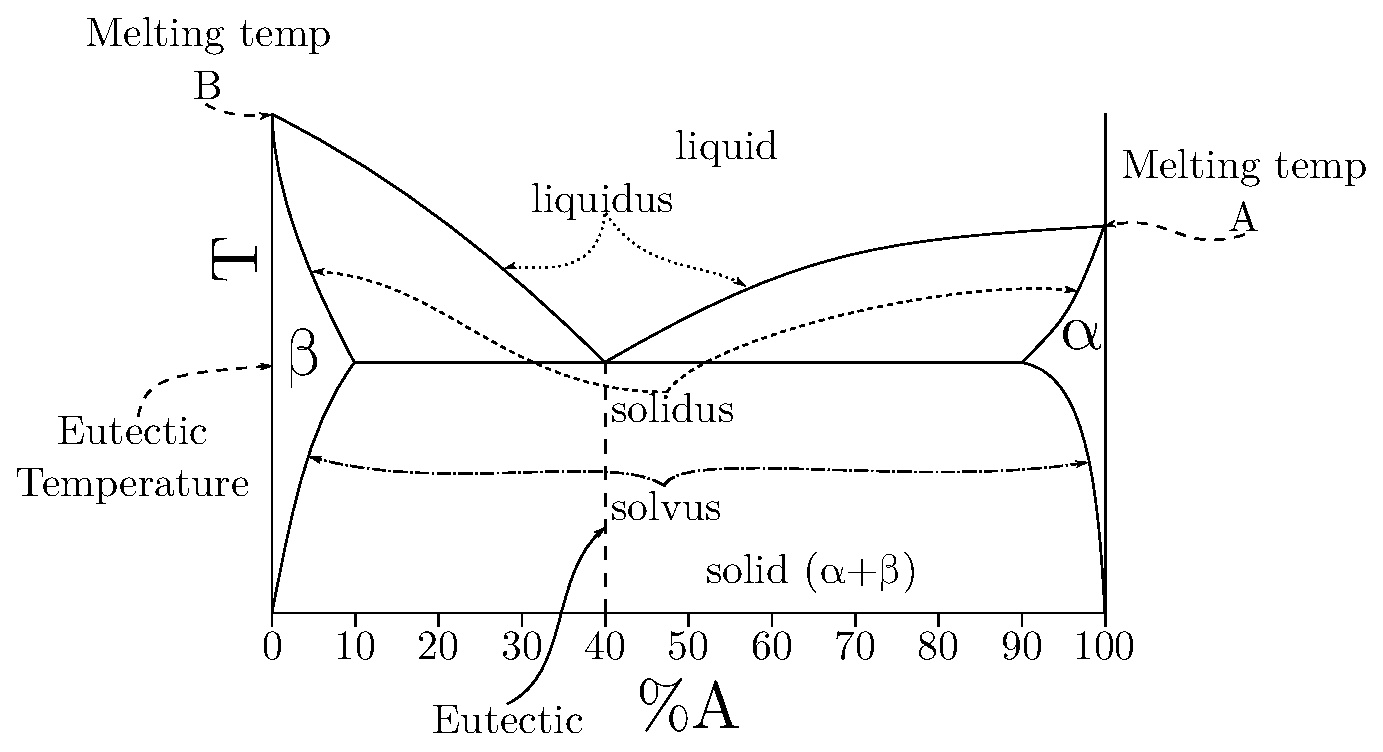
\includegraphics[width=\linewidth]{pdab.eps}
		\caption{Binary phase diagram. Eutectic 40\% A, liquid and solid regions, liquidus, solvus and solidus lines, melting temperatures of A and B, eutectic temperature and solubility limits.}
		\label{f:pdab}
	\end{figure}
	\subsection{e)}
	\Cref{f:abe} shows sketches of the Gibbs free energy for the system in \cref{ss:pdab} at just above (\cref{sf:abht}) and below (\cref{sf:ablt}) the eutectic temperature.
	\begin{figure}
		\centering
		\begin{subfigure}[b]{\linewidth}
			\centering
			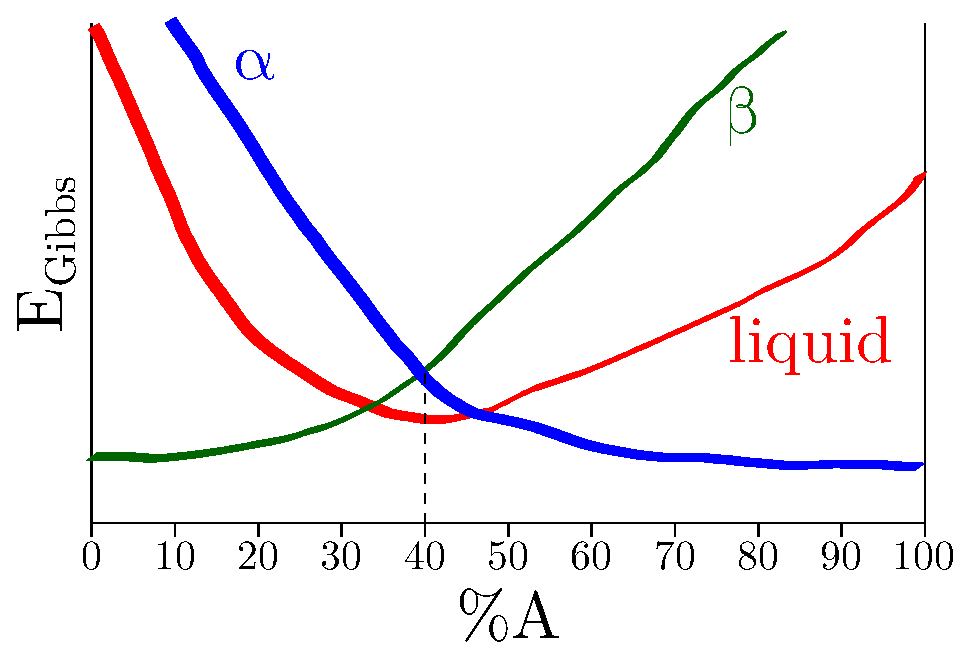
\includegraphics[width=\linewidth]{abht.eps}
			\caption{Just above the eutectic temperature.}
			\label{sf:abht}
		\end{subfigure}
		
		\begin{subfigure}[b]{\linewidth}
			\centering
			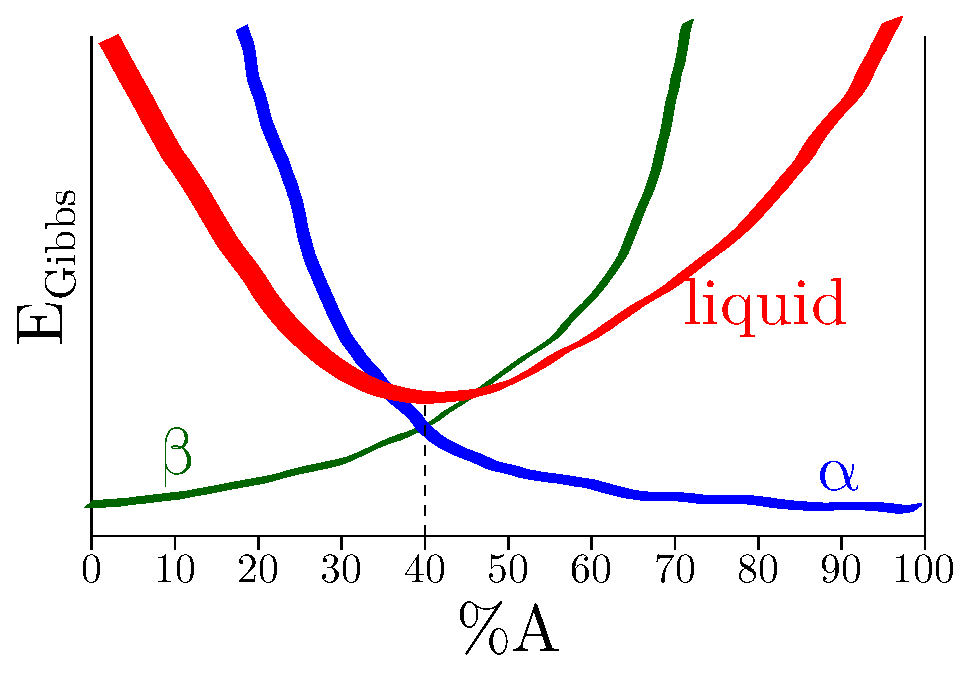
\includegraphics[width=\linewidth]{ablt.eps}
			\caption{Just below the eutectic temperature.}
			\label{sf:ablt}
		\end{subfigure}
		\caption{Sketches of the Gibbs free energies of the binary system in \cref{ss:pdab}.}
	\end{figure}
\end{document}